\section*{Appendix: Bootstrap Distributions and Normality Checks}
\label{sec:appendix_bootstrap}

% ==========================================
% Model 1 (Base Model)
% ==========================================
\subsection*{A.1 Model 1}

\begin{figure}[htbp]
    \centering
    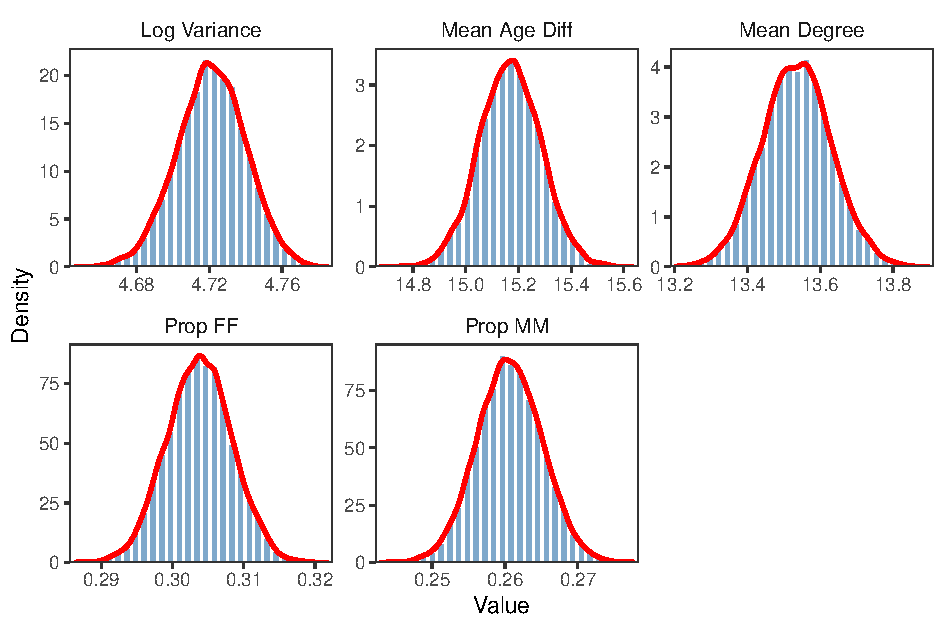
\includegraphics[width=0.9\textwidth]{figures/06_Appendix/density_bootstrap_m1.pdf}
    \caption{Density plots of the bootstrapped summary statistics for Model 1. The histograms represent the distribution of 10,000 bootstrap samples, overlaid with the estimated density curves (red lines).}
    \label{fig:density_m1}
\end{figure}

\begin{figure}[htbp]
    \centering
    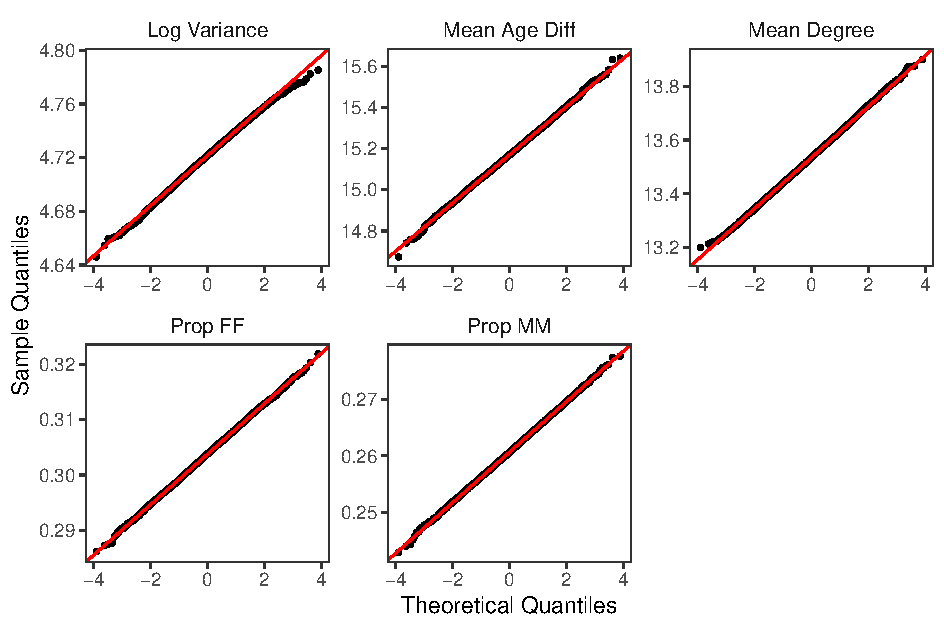
\includegraphics[width=0.9\textwidth]{figures/06_Appendix/qqplot_bootstrap_m1.pdf}
    \caption{QQ plots of the bootstrapped summary statistics for Model 1. The sample quantiles closely matching the theoretical normal quantiles (red lines) indicate that the statistics are approximately normally distributed.}
    \label{fig:qq_m1}
\end{figure}

\clearpage

% ==========================================
% Model 2A
% ==========================================
\subsection*{A.2 Model 2A}

\begin{figure}[htbp]
    \centering
    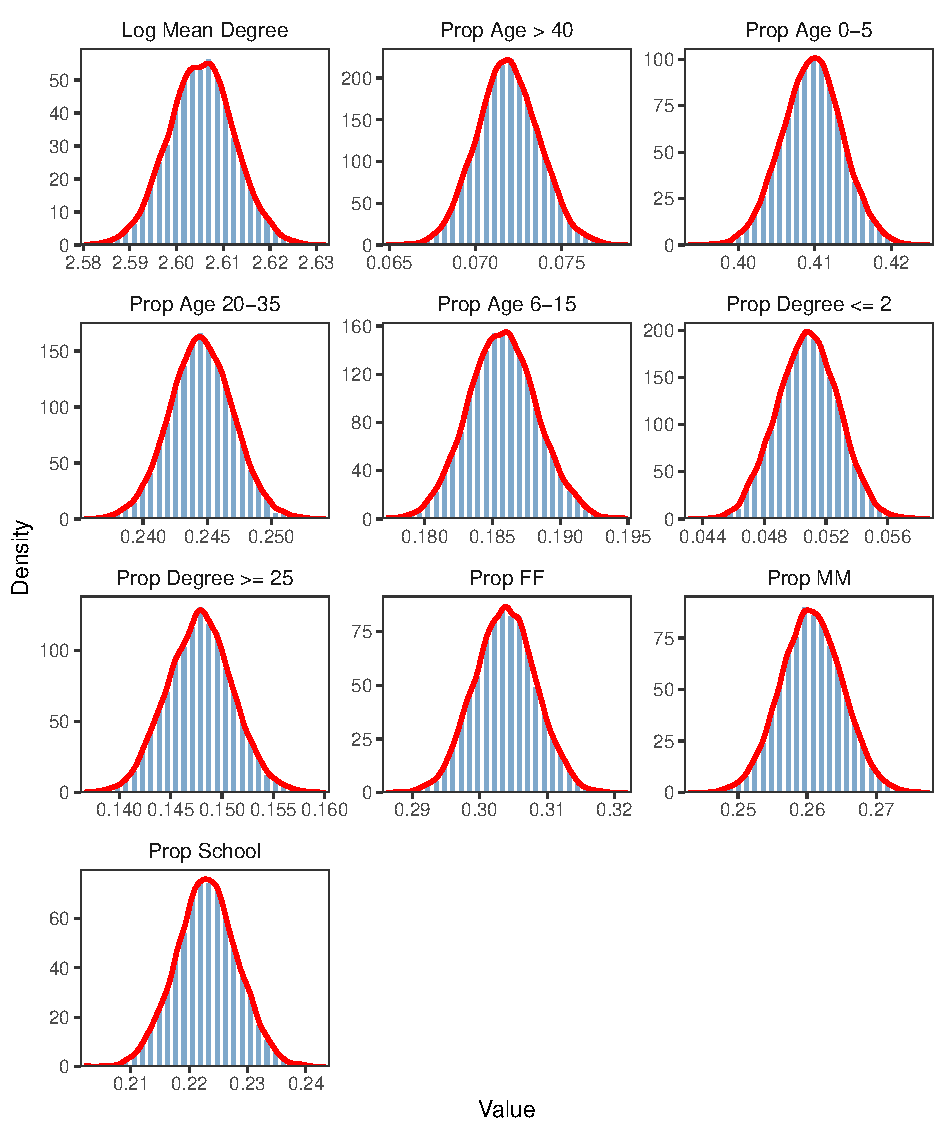
\includegraphics[width=0.85\textwidth]{figures/06_Appendix/density_bootstrap_m2a.pdf}
    \caption{Density plots of the bootstrapped summary statistics for Model 2A (10 variables).}
    \label{fig:density_m2a}
\end{figure}

\begin{figure}[htbp]
    \centering
    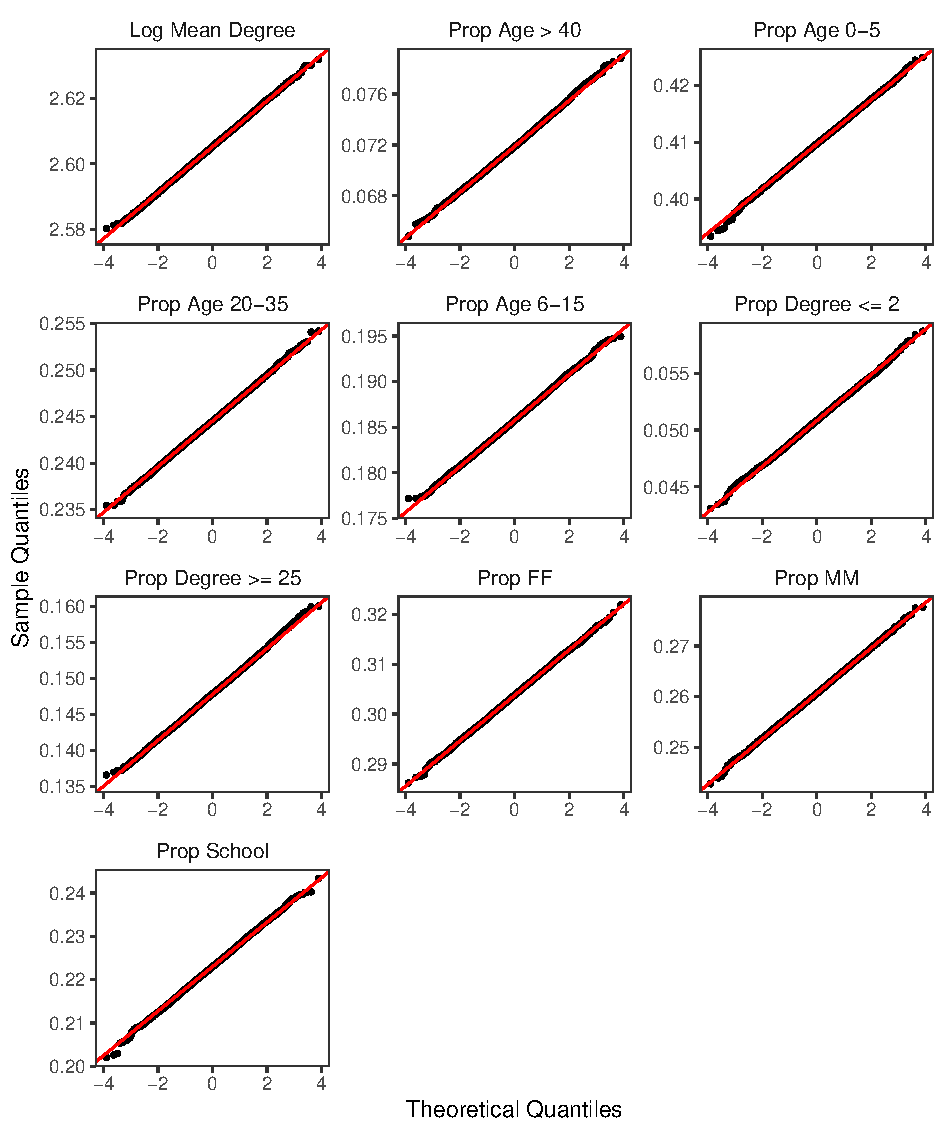
\includegraphics[width=0.85\textwidth]{figures/06_Appendix/qqplot_bootstrap_m2a.pdf}
    \caption{QQ plots of the bootstrapped summary statistics for Model 2A.}
    \label{fig:qq_m2a}
\end{figure}

\clearpage

% ==========================================
% Model 2B
% ==========================================
\subsection*{A.3 Model 2B}

\begin{figure}[htbp]
    \centering
    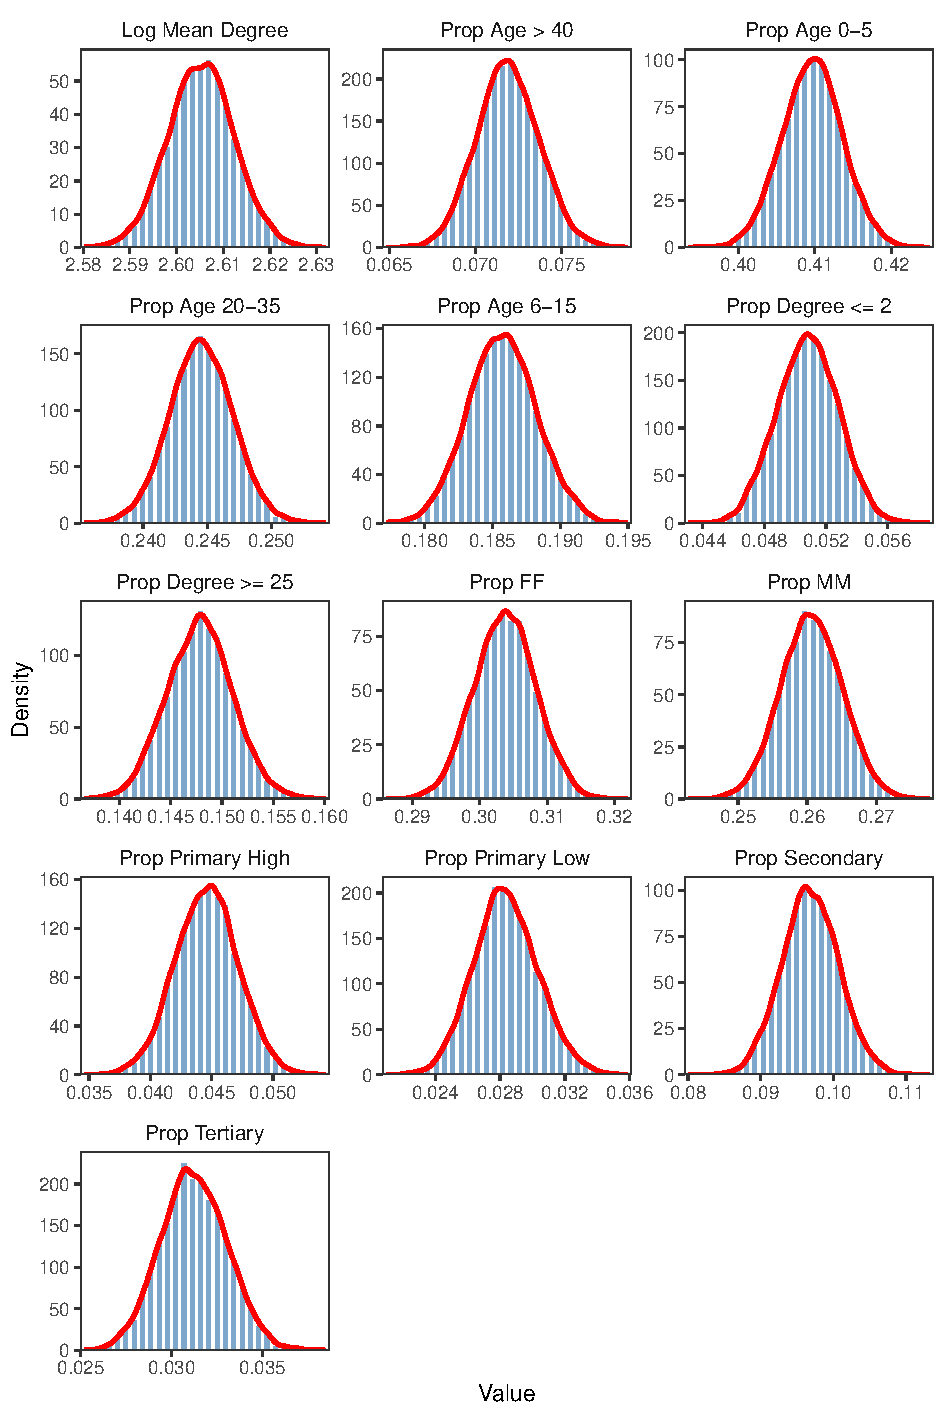
\includegraphics[width=0.7\linewidth]{figures/06_Appendix/density_bootstrap_m2b.pdf}
    \caption{Density plots of the bootstrapped summary statistics for Model 2B (13 variables).}
    \label{fig:density_m2b}
\end{figure}

\begin{figure}[htbp]
    \centering
    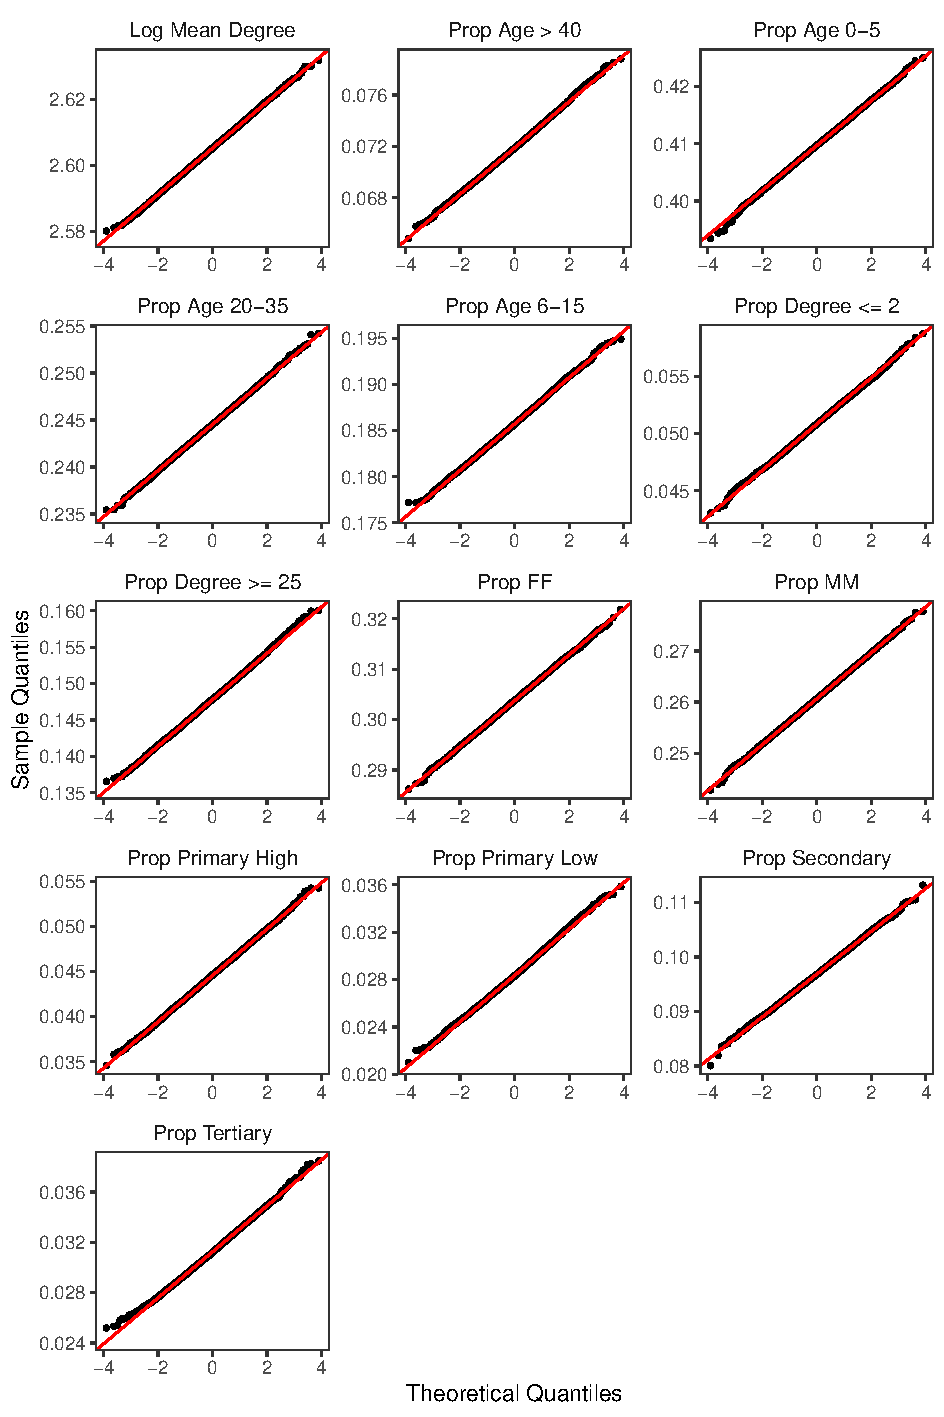
\includegraphics[width=0.7\textwidth]{figures/06_Appendix/qqplot_bootstrap_m2b.pdf}
    \caption{QQ plots of the bootstrapped summary statistics for Model 2B.}
    \label{fig:qq_m2b}
\end{figure}

\clearpage

\section*{Appendix: MCMC Trace Plots}
\label{sec:appendix_traceplots}

% ==========================================
% Model 1
% ==========================================
\subsection*{B.1 Model 1}

\begin{figure}[htbp]
    \centering
    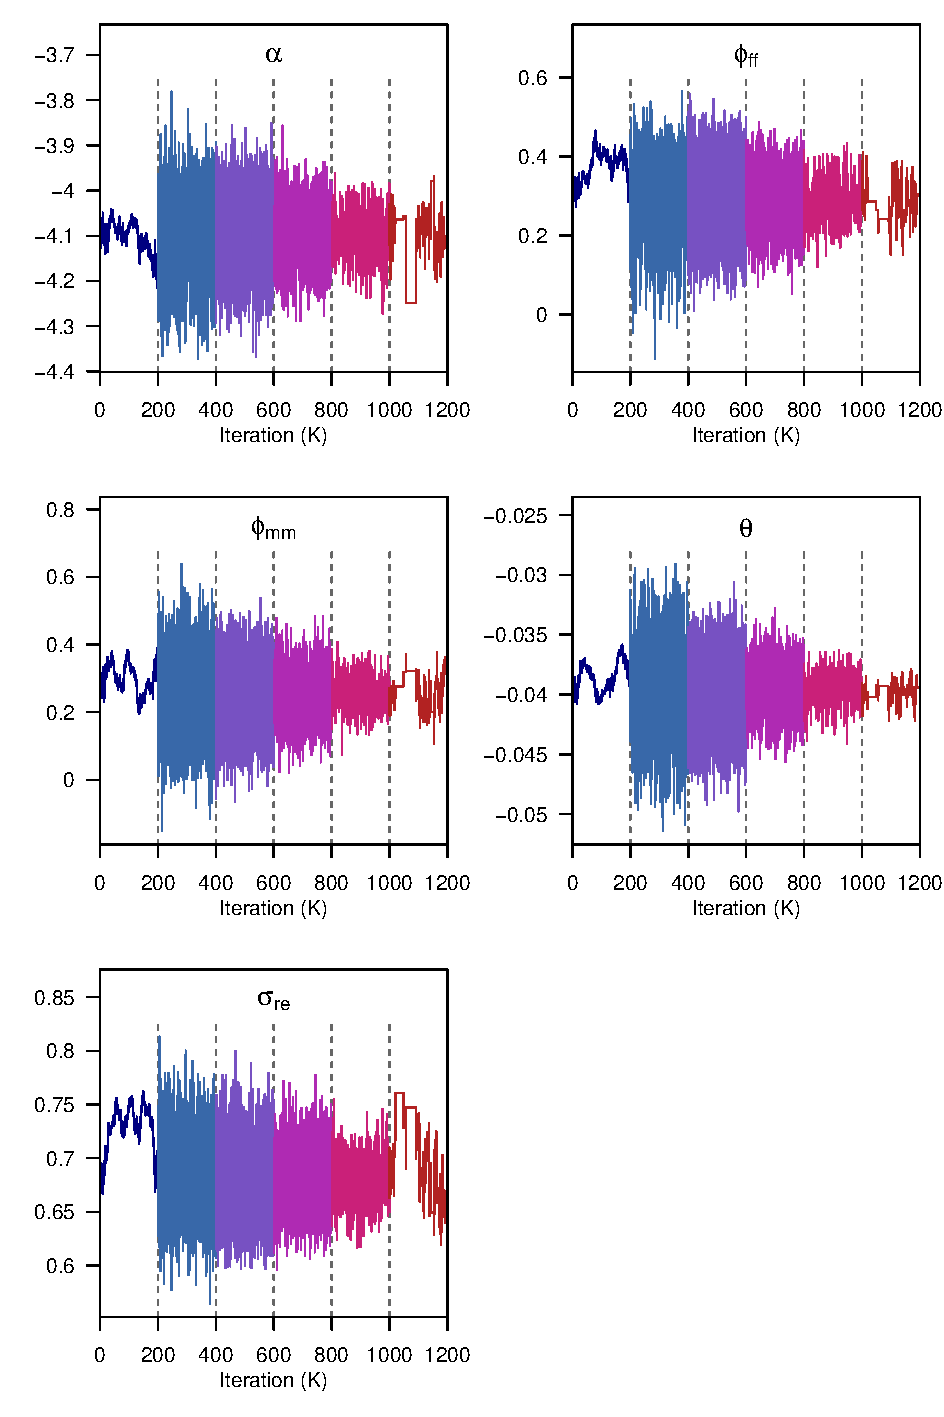
\includegraphics[width=0.75\textwidth]{figures/06_Appendix/model1_multistage_traceplot_1.pdf}
    \caption{Model 1: Multistage MCMC trace plots.}
    \label{fig:trace_m1_multi}
\end{figure}

\begin{figure}[htbp]
    \centering
    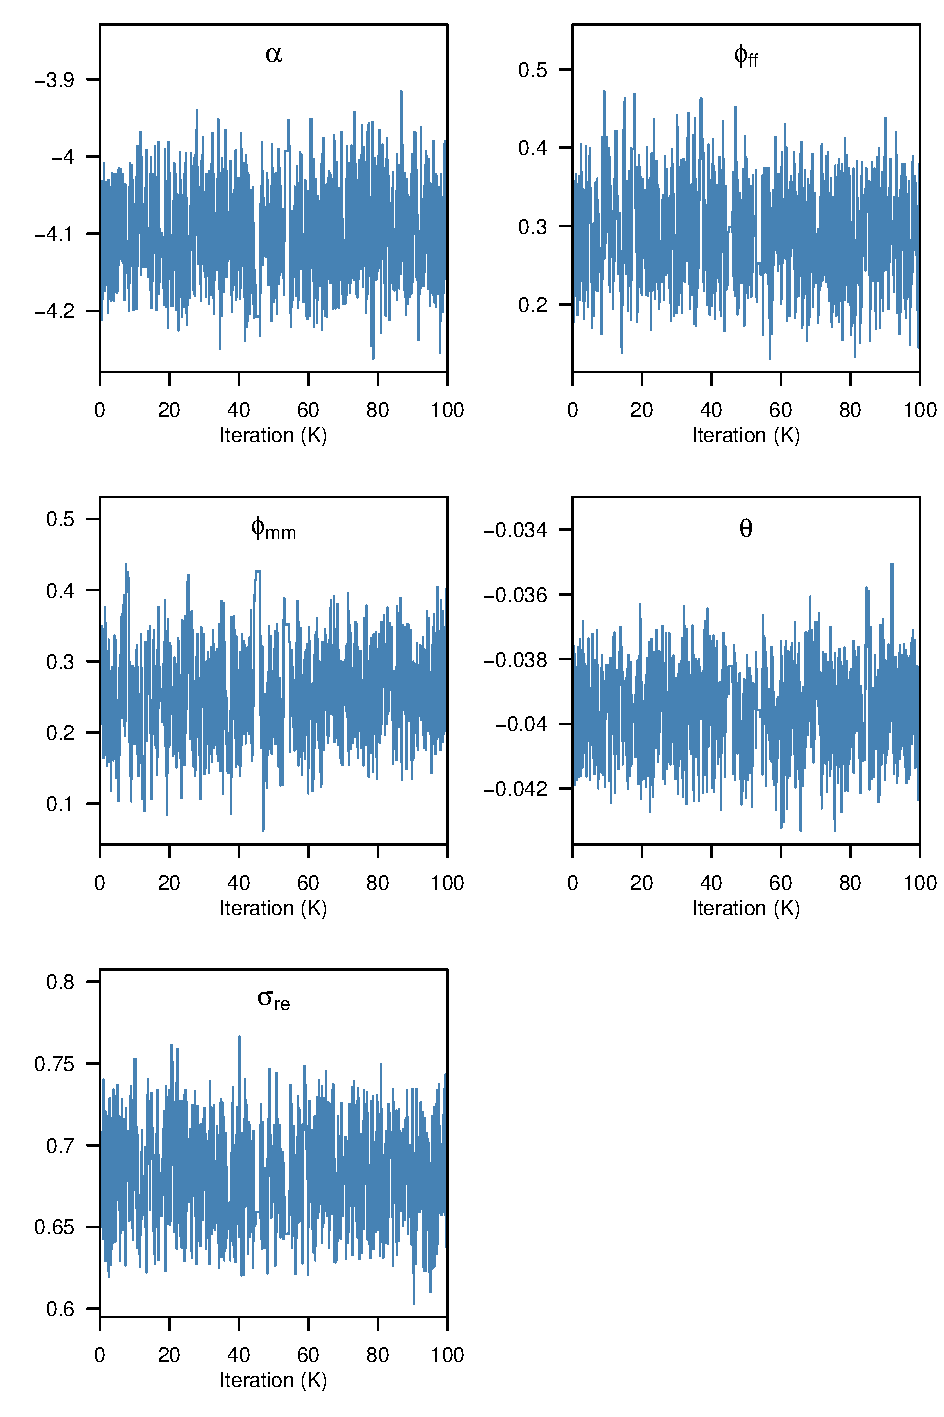
\includegraphics[width=0.85\textwidth]{figures/06_Appendix/model1_singlestage_traceplot_1.pdf}
    \caption{Model 1: Singlestage MCMC trace plots.}
    \label{fig:trace_m1_single}
\end{figure}

\clearpage

% ==========================================
% Model 2A
% ==========================================
\subsection*{B.2 Model 2A}

\begin{figure}[htbp]
    \centering
    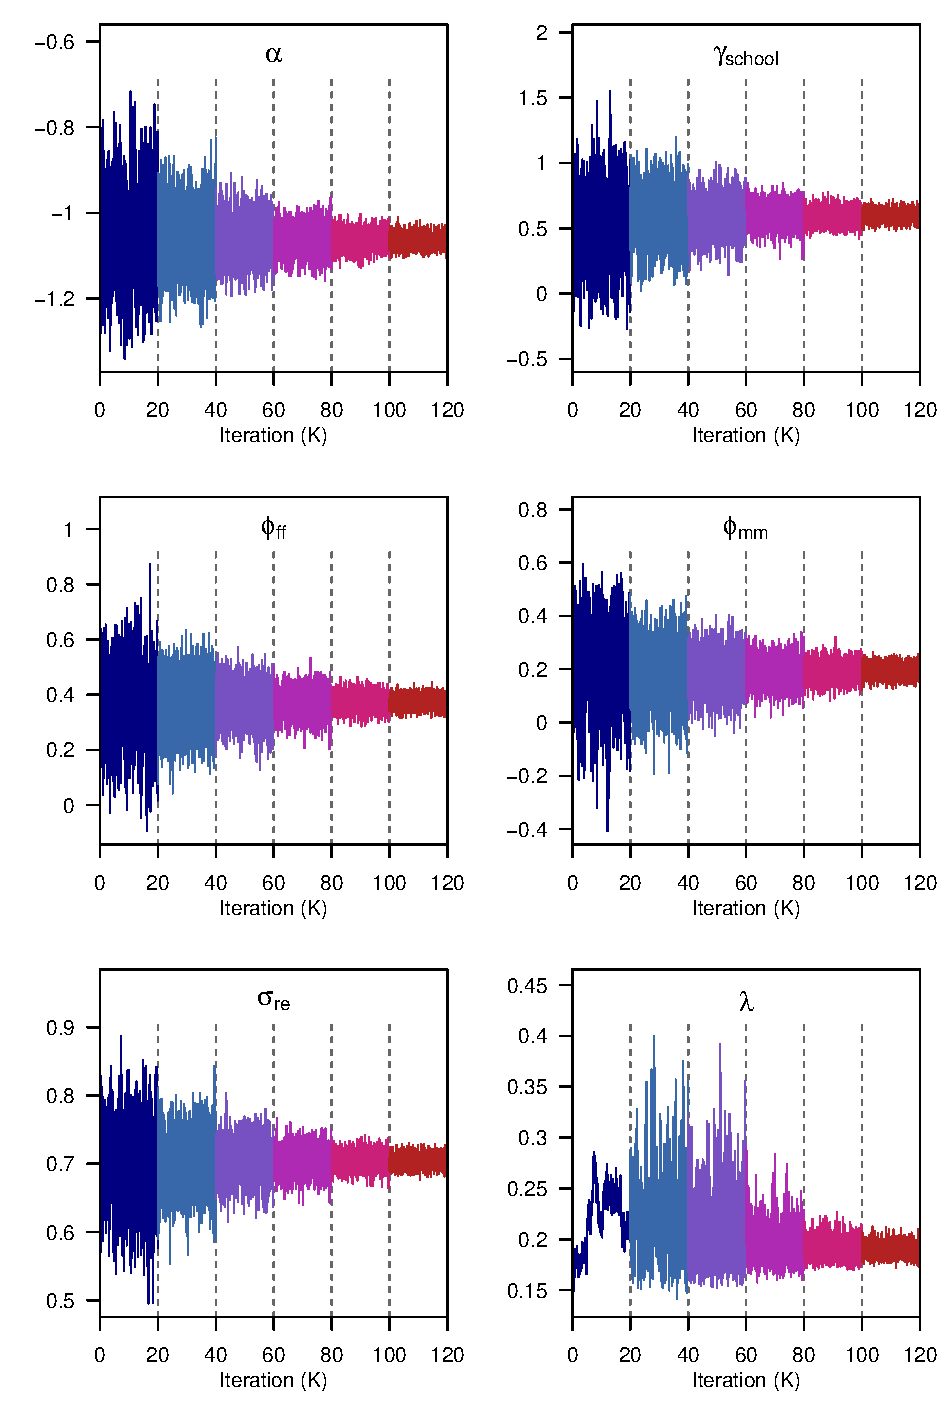
\includegraphics[width=0.75\textwidth]{figures/06_Appendix/model2a_multistage_traceplot_1.pdf}
\end{figure}
\begin{figure}[htbp]
    \centering
    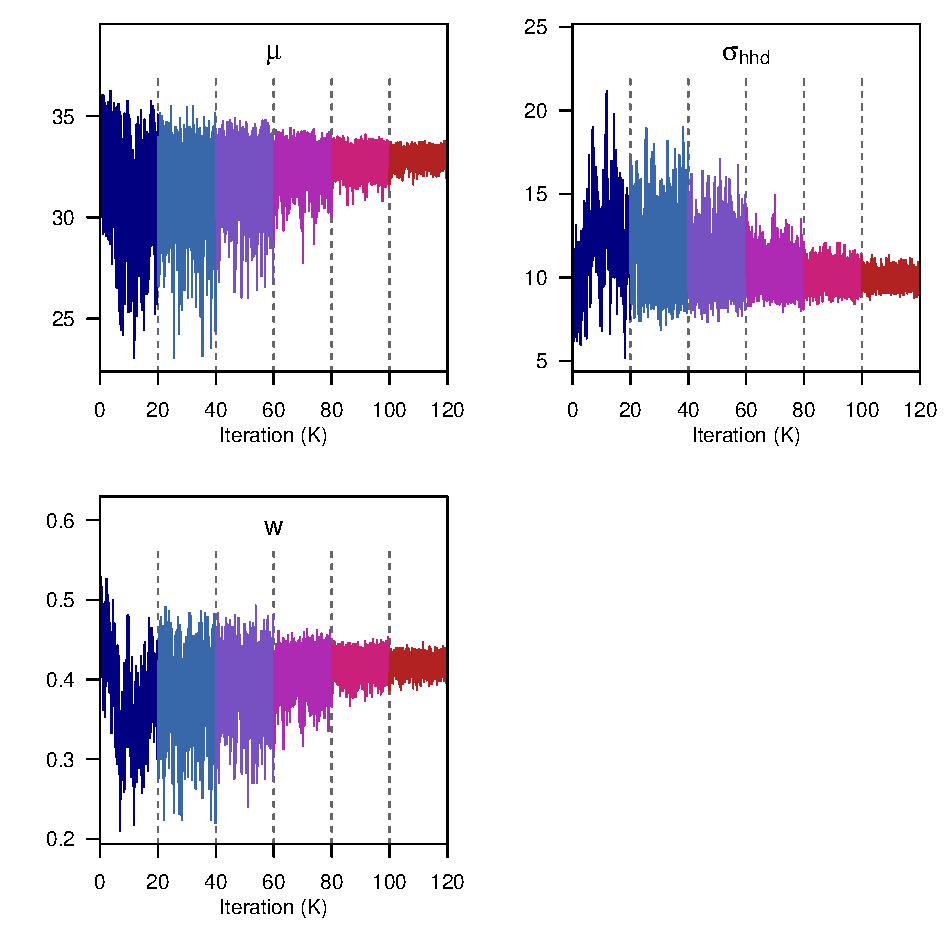
\includegraphics[width=0.75\textwidth]{figures/06_Appendix/model2a_multistage_traceplot_2.pdf}
    \caption{Model 2A: Multistage MCMC trace plots (Set 1 and 2).}
    \label{fig:trace_m2a_multi}
\end{figure}


\begin{figure}[htbp]
    \centering
    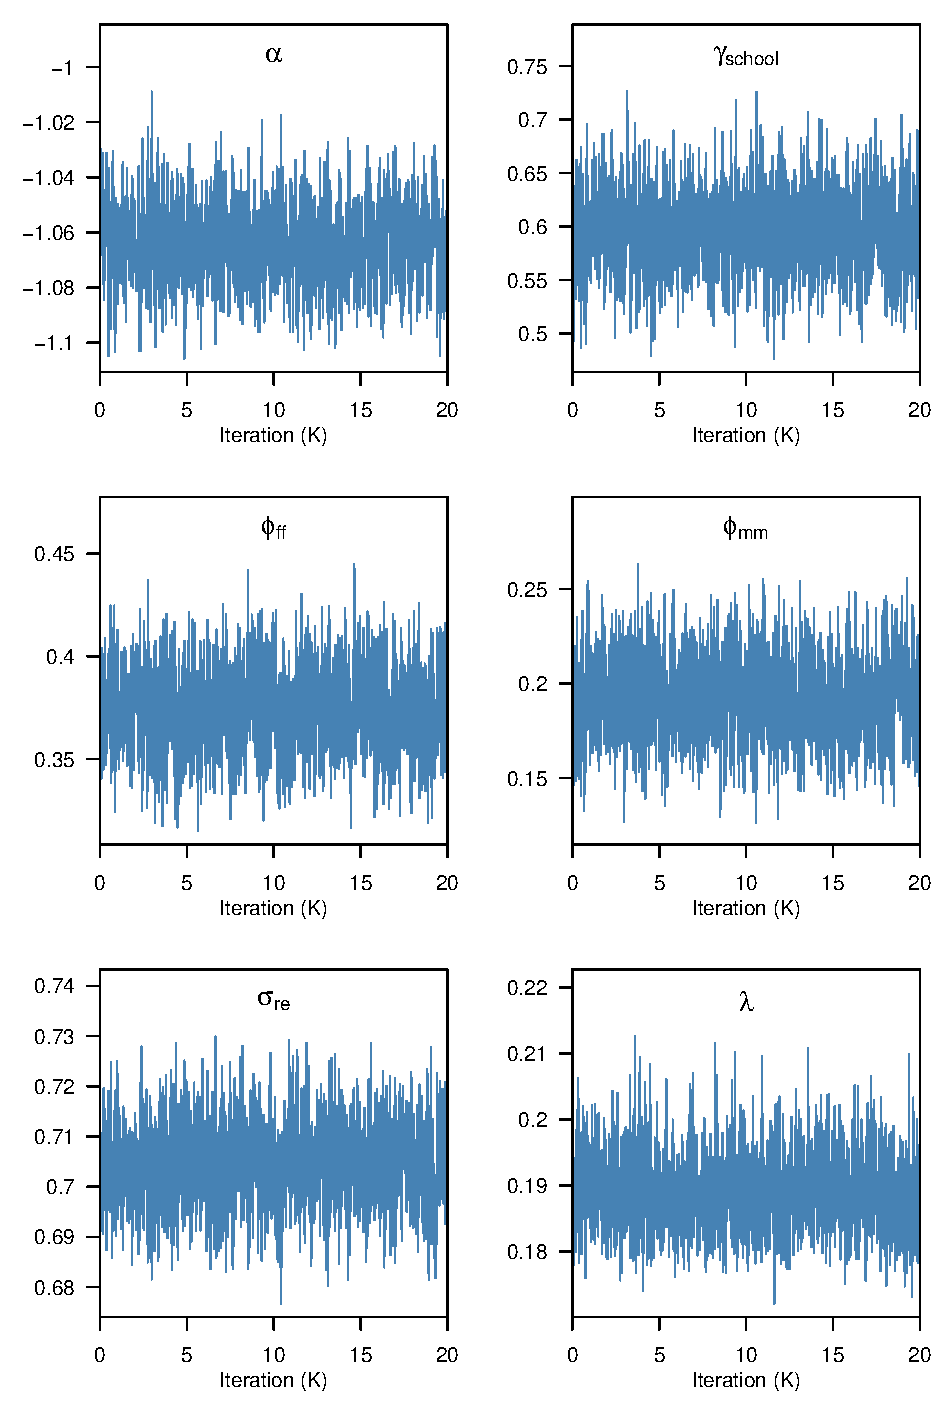
\includegraphics[width=0.75\textwidth]{figures/06_Appendix/model2a_singlestage_traceplot_1.pdf}
\end{figure}
\begin{figure}[htbp]
    \centering
    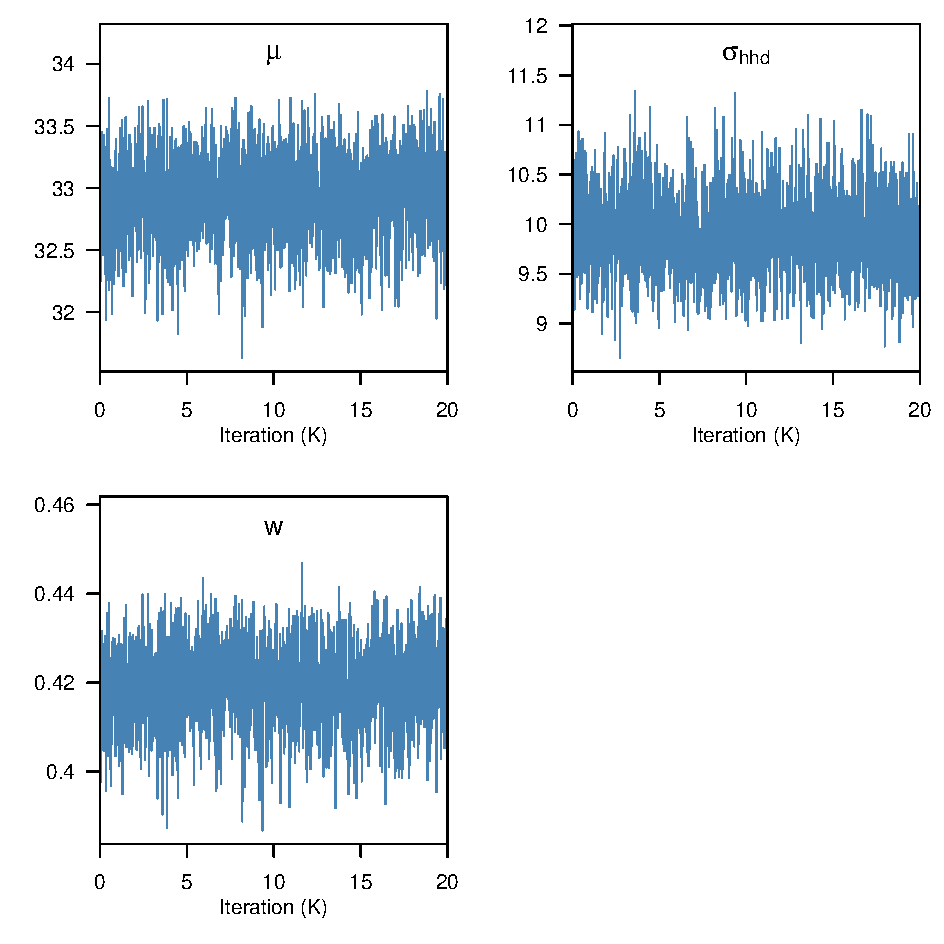
\includegraphics[width=0.75\textwidth]{figures/06_Appendix/model2a_singlestage_traceplot_2.pdf}
    \caption{Model 2A: Singlestage MCMC trace plots (Set 1 and 2).}
    \label{fig:trace_m2a_single}
\end{figure}

\clearpage

% ==========================================
% Model 2B
% ==========================================
\subsection*{B.3 Model 2B}

\begin{figure}[htbp]
    \centering
    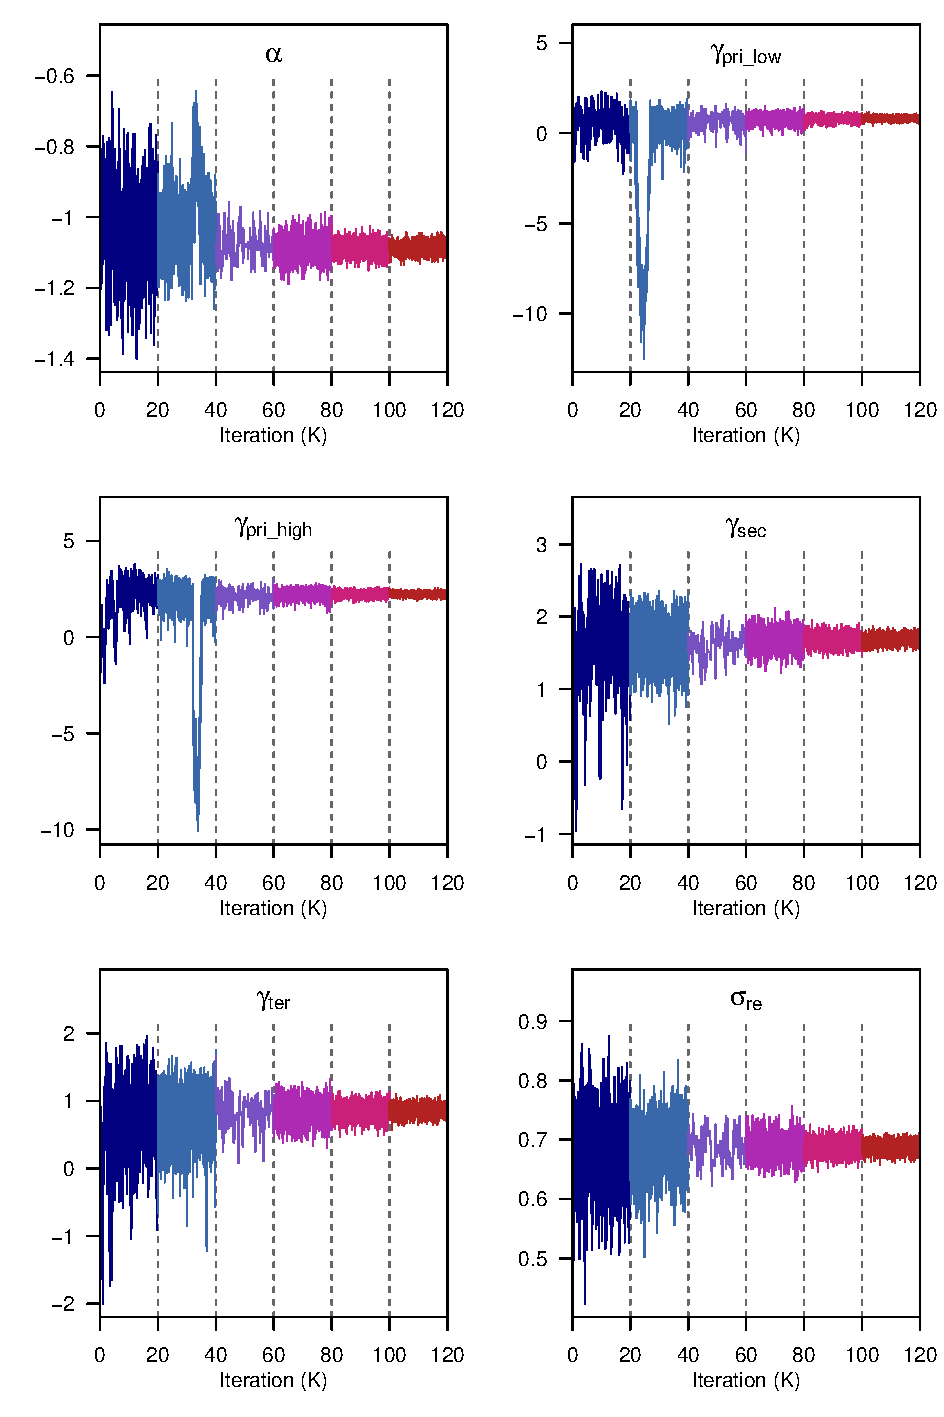
\includegraphics[width=0.75\textwidth]{figures/06_Appendix/model2b_multistage_traceplot_1.pdf}
\end{figure}
\begin{figure}[htbp]
    \centering
    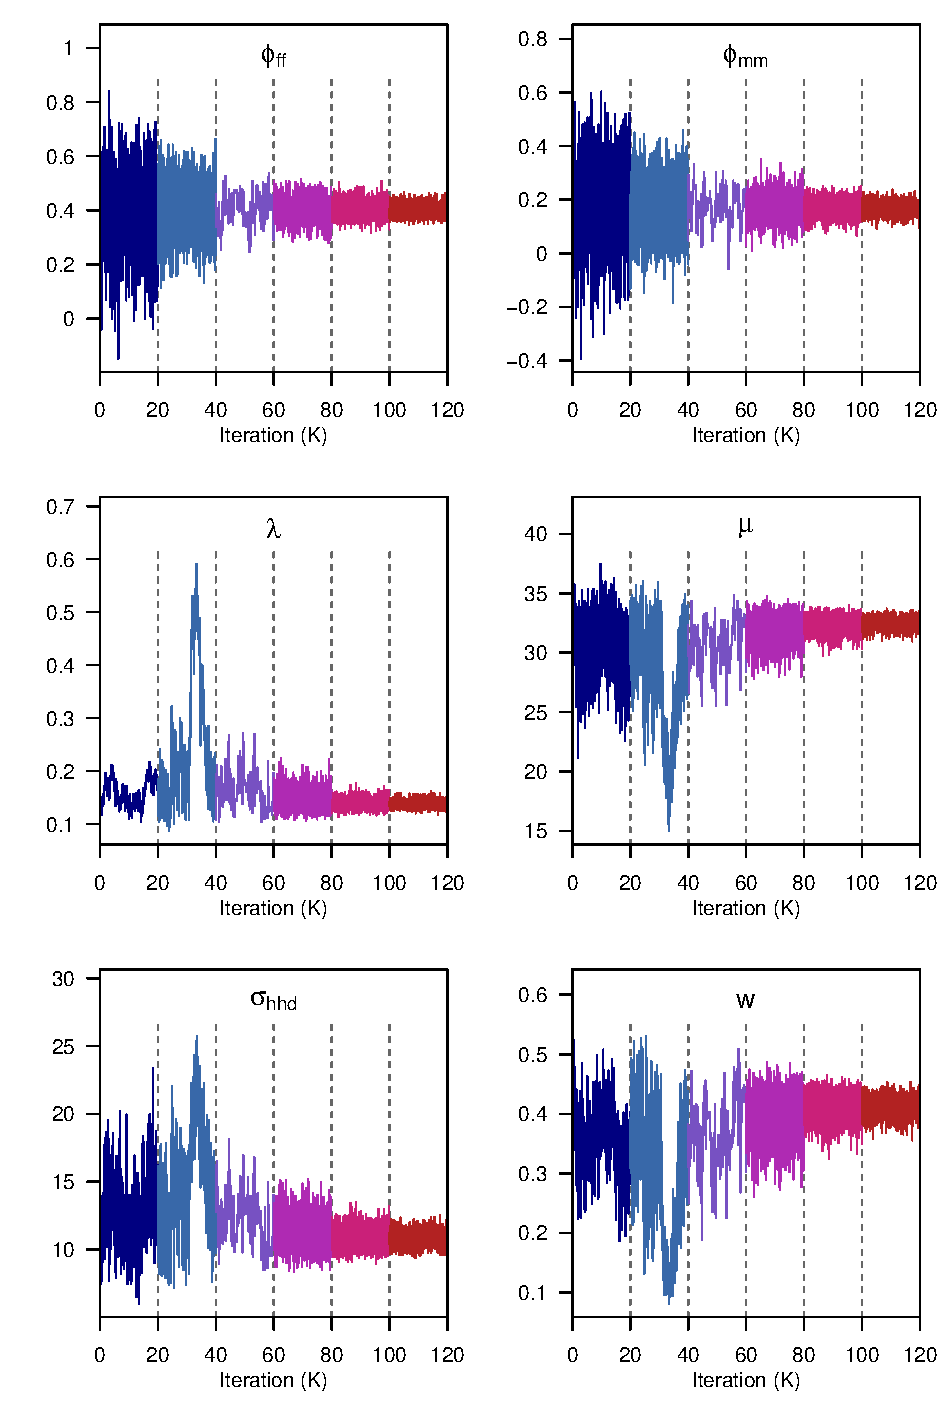
\includegraphics[width=0.75\textwidth]{figures/06_Appendix/model2b_multistage_traceplot_2.pdf}
    \caption{Model 2B: Multistage MCMC trace plots (Set 1 and 2).}
    \label{fig:trace_m2b_multi}
\end{figure}

\begin{figure}[htbp]
    \centering
    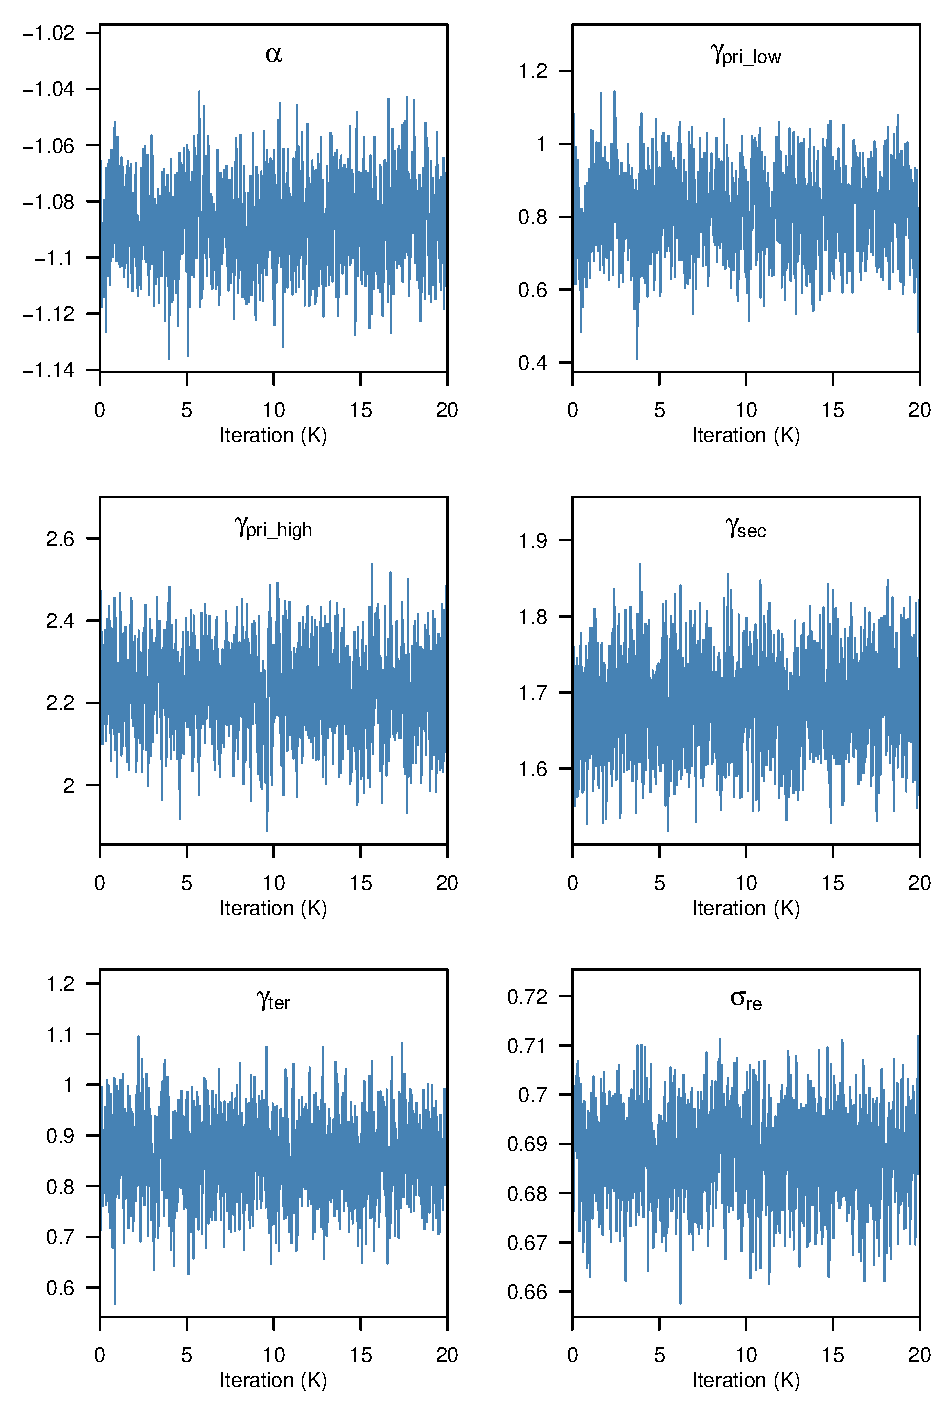
\includegraphics[width=0.75\textwidth]{figures/06_Appendix/model2b_singlestage_traceplot_1.pdf}
\end{figure}
\begin{figure}[htbp]
    \centering
    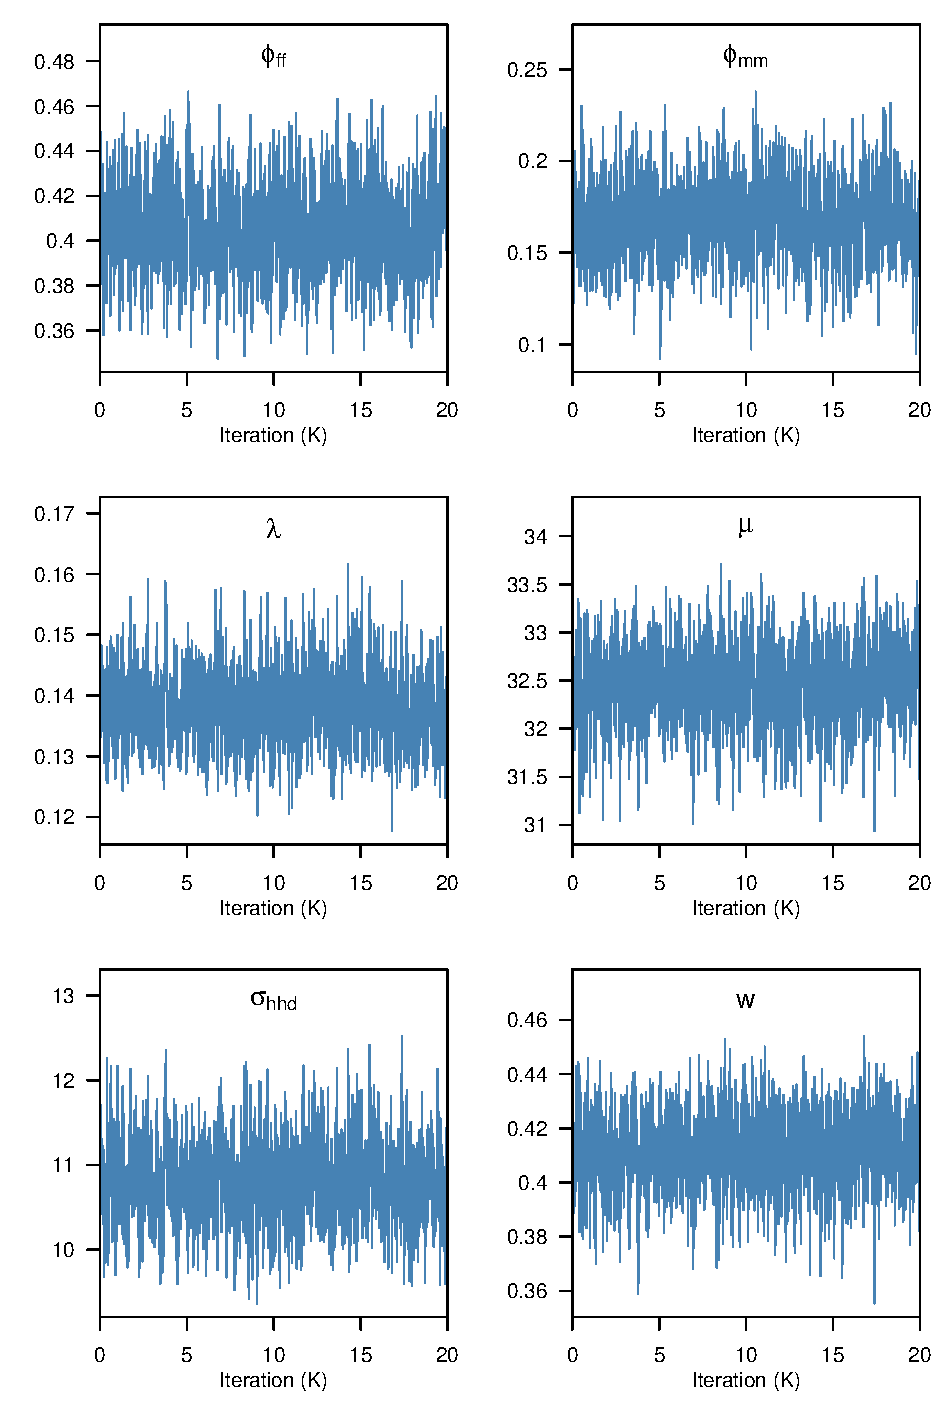
\includegraphics[width=0.75\textwidth]{figures/06_Appendix/model2b_singlestage_traceplot_2.pdf}
    \caption{Model 2B: Singlestage MCMC trace plots (Set 1 and 2).}
    \label{fig:trace_m2b_single}
\end{figure}

\clearpage


\section*{Appendix: Comparison of Summary Statistics}
\label{sec:appendix_stats_comparison}


% ==========================================
% Model 1
% ==========================================
\subsection*{C.1 Model 1: Summary Statistics Comparison}

\begin{table}[htbp]
    \centering
    \caption{Comparison of summary statistics for Model 1 (Base Model). The Z-score measures the deviation of the target from the simulation mean in units of simulation standard deviation.}
    \label{tab:stats_m1}
    \small
    \begin{tabular}{lcccccc}
        \toprule
        Statistic & Target Mean & Sim Mean & Z-Score & Sim 95\% Lower & Sim 95\% Upper \\
        \midrule
        Mean Degree   & 13.535 & 13.667 & -0.129 & 11.905 & 16.005 \\
        Log Variance  & 4.721  & 4.746  & -0.127 & 4.398  & 5.157 \\
        Mean Age Diff & 15.169 & 15.160 & 0.030  & 14.633 & 15.709 \\
        Prop MM       & 0.261  & 0.260  & 0.059  & 0.222  & 0.296 \\
        Prop FF       & 0.304  & 0.306  & -0.098 & 0.267  & 0.348 \\
        \bottomrule
    \end{tabular}
\end{table}

% ==========================================
% Model 2A
% ==========================================
\subsection*{C.2 Model 2A: Summary Statistics Comparison}

\begin{table}[htbp]
    \centering
    \caption{Comparison of summary statistics for Model 2A (Matrix model v4.2).}
    \label{tab:stats_m2a}
    \small
    \begin{tabular}{lcccccc}
        \toprule
        Statistic & Target Mean & Sim Mean & Z-Score & Sim 95\% Lower & Sim 95\% Upper \\
        \midrule
        Log Mean Degree      & 2.605 & 2.587 & 2.600 & 2.574 & 2.600 \\
        Prop Degree $\le$ 2  & 0.051 & 0.060 & -5.312 & 0.057 & 0.064 \\
        Prop Degree $\ge$ 25 & 0.148 & 0.117 & 13.591 & 0.113 & 0.121 \\
        Prop MM              & 0.261 & 0.265 & -0.856 & 0.256 & 0.273 \\
        Prop FF              & 0.304 & 0.301 & 0.499 & 0.293 & 0.310 \\
        Prop Age 0-5         & 0.410 & 0.410 & -0.050 & 0.403 & 0.417 \\
        Prop Age 6-15        & 0.186 & 0.185 & 0.182 & 0.181 & 0.190 \\
        Prop Age 20-35       & 0.245 & 0.235 & 4.019 & 0.231 & 0.240 \\
        Prop Age $> 40$      & 0.072 & 0.067 & 2.971 & 0.063 & 0.070 \\
        Prop School          & 0.223 & 0.223 & -0.022 & 0.213 & 0.233 \\
        \bottomrule
    \end{tabular}
\end{table}

\clearpage

% ==========================================
% Model 2B
% ==========================================
\subsection*{C.3 Model 2B: Summary Statistics Comparison}

\begin{table}[htbp]
    \centering
    \caption{Comparison of summary statistics for Model 2B (Refined school structure).}
    \label{tab:stats_m2b}
    \footnotesize
    \begin{tabular}{lcccccc}
        \toprule
        Statistic & Target Mean & Sim Mean & Z-Score & Sim 95\% Lower & Sim 95\% Upper \\
        \midrule
        Log Mean Degree      & 2.605 & 2.592 & 1.898 & 2.577 & 2.606 \\
        Prop Degree $\le$ 2  & 0.051 & 0.059 & -4.338 & 0.055 & 0.062 \\
        Prop Degree $\ge$ 25 & 0.148 & 0.123 & 11.262 & 0.118 & 0.127 \\
        Prop MM              & 0.261 & 0.259 & 0.284 & 0.250 & 0.269 \\
        Prop FF              & 0.304 & 0.307 & -0.765 & 0.298 & 0.316 \\
        Prop Age 0-5         & 0.410 & 0.412 & -0.554 & 0.405 & 0.419 \\
        Prop Age 6-15        & 0.186 & 0.184 & 0.813 & 0.179 & 0.188 \\
        Prop Age 20-35       & 0.245 & 0.232 & 5.534 & 0.227 & 0.236 \\
        Prop Age $> 40$      & 0.072 & 0.065 & 3.575 & 0.062 & 0.069 \\
        Prop Primary Low     & 0.028 & 0.025 & 1.653 & 0.021 & 0.029 \\
        Prop Primary High    & 0.045 & 0.042 & 0.792 & 0.037 & 0.048 \\
        Prop Secondary       & 0.097 & 0.102 & -1.457 & 0.095 & 0.109 \\
        Prop Tertiary        & 0.031 & 0.032 & -0.374 & 0.029 & 0.035 \\
        \bottomrule
    \end{tabular}
\end{table}